
\فصل{کارهای پیشین}
این بخش را می‌توان به دو قسمت پیشینه کارهای انجام شده در استفاده از تئوری بازی در کنترل سیستم و حوزه کنترل چهارپره 
تقسیم‌بندی کرد. که در دو بخش \ref{gameControl} و بخش \ref{QuadControl} ارائه شده‌است.
\section{کنترل‌کننده مبتنی بر تئوری بازی}\label{gameControl}
%\begin{figure}[H]\label{LabQuad}
%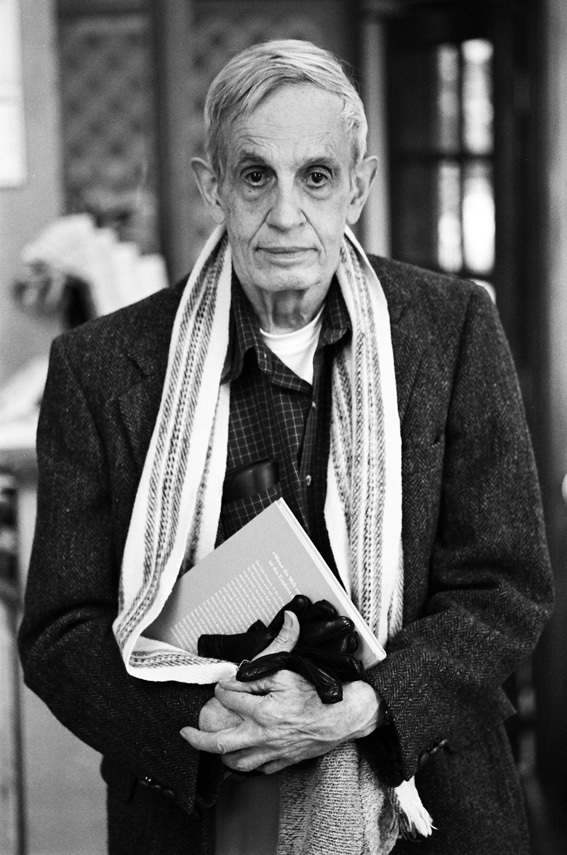
\includegraphics[width=6cm]{figs/introduction/John_Forbes_Nash,_Jr._by_Peter_Badge.jpg}
%\centering
%\caption{جان فوربز نش\cite{JanNash}}
%\end{figure}
در منبع \cite{article1} به صورت خلاصه نظریه بازی و تعادل نش توضیح داده شده‌است. در حالتی از تئوری بازی می‌توان با دیگر بازیکنان همکاری یا رقابت کرد که در منیع\cite{8376282} یرای یک پهباد\LTRfootnote{UAC(unmanned aerial vehicle)} بررسی شده است. به علت اینکه هدف هر بازیکن افزایش امتیاز خود و کاهش امتیاز رقیب هست، این مسئله از نوع غیرمشارکتی\LTRfootnote{non-cooperative} در نظر گرفته شده‌است. در این مسئله دو معادله دیفرانسیل شروع به بازی با یکدیگر می‌کنند که هدف هر کدام افزایش امتیاز خود است. در روش کنترل کننده خطی مبتنی بر بازی دیفرانسیلی یک تابع هزینه برای هر بازیکن ایجاد می‌شود. این مسائل فرض شده که اطلاعات در اختیار تمامی بازیکنان قرار دارد و هیچ یک از آینده خبر ندارند.

از کابردهای بازی دیفرانسیلی می‌توان به فرود بر روی اجسام متحرک مانند فرود چهارپره، هلیکوپتر و پهباد بر روی ناو\cite{8996044} اشاره کرد. در منبع \cite{9001045} از تئوری بازی و بازی دیفرانسیلی برای نبرد بین دو پهباد استفاده شده‌است. قدرت تئوری بازی بر تحلیل رفتارهای دو یا چندین بازیکن است بر همین اساس در منبع \cite{Pachter2019} برای دفاع و بررسی تحدید بازیکنان دیگر و در منبع \cite{7502594} از کنترل کننده خطی برای شکل پرواز گروه سه نفره از پهبادها استفاده شده‌است. بازی دیفرانسیلی در ناوبری کاردبرد ویژه‌ای دارد، در منبع \cite{6160198} از این روش برای هدایت و ناوبری یک میکروپهباد\LTRfootnote{Micro-UAV (MAV)} استفاده شده‌است. در منبع \cite{1595165} از بازی دیفرانسیلی برای گشت و گریز پهباها استفاده شده‌است.

تابع هزینه در این مسائل بسیار شبیه به کنترل‌کننده بهینه خطی\LTRfootnote{LQR} است. در منبع \cite{4399042} از روش کنترل‌کننده بهینه خطی برای کنترل وضعیت یک چهارپره استفاده شده‌است. در منبع \cite{article2} شراط وجود جواب و حل معادلات ریکاتی \LTRfootnote{Riccati} LQDG ارائه شده‌است. در این کنترل‌کننده احتیاج به مدل سیستم است.
\section{کنترل چهارپره}\label{QuadControl}
کنترل به روش LQR یکی از متداول‌ترین روش‌های کنترل چهارپره است.
در منبع \cite{8394911} از روش LQR برای ردیابی مسیر یک نقطه  \LTRfootnote{Tracking} با چهارپره استفاده شده و در آخر نتایج شبیه‌سازی با کنترل کننده تناسبی-انتگرالی-مشتقی مقایسه شد‌ه‌است. 
در سال 2014 توسط Mueller و D’Andrea یک روش برای کنترل چهارپره با از دست دادن کامل یک، دو و سه پره توسعه داده‌شد که اساس اجرای آن روش LQR بود\cite{6906588}.

در منابع \cite{Lee2017} \cite{8396617} یک روش مسریابی بهینه برای چندپره‌ها از جمله چهارپره طراحی شده‌است. چهارپره‌ها انرژی محدودی دارند برای همین مشکل در منبع \cite{9029345} یک بهینه سازی بر روی انرژی چهارپره که در مسیر جنگلی حرکت می‌کند، انجام شده‌است. در مواری \cite{DBLP:journals/corr/abs-1912-07067}از کنترل بهینه و یادگیری عمیق \LTRfootnote{Deep Learning} برای پایداری چهارپره استفاده شده‌است.

